\chapter{Implementierung}
\label{chap:implementation}
% TODO: Dieses Kaptiel mit der Zeit anpassen

\section{Unity Engine}
\emph{Unity} \autocite{UnityTechnologies2018} ist eine \emph{Engine} zum Entwickeln von 2D- und 3D-Anwendung (vornehmlich Spiele).
Da Unity plattformunabhängig ist werden die Applikationen gleichzeitig für mehrere Plattformen entwickelt.
Erstellt werden die Anwendungen mit dem Unity Editor.

Eine Unity-Anwendung ist in Szenen unterteilt.
Jede Szene besitzt einen eigenen Szenengraph.
Dieser Graph verwaltet alle Objekte einer Szene.
Unity verwendet ein Entitäten-Komponenten-System.
Das heißt, alle Unity-Objekte sind im Kern attribut- und funktionslose Entitäten (in Unity \emph{GameObject}s genannt).
Die eigentliche Funktionalität wird erst durch Hinzufügen von Komponenten (\emph{Components}) zu den GameObjects deutlich.
Beispielsweise verfügt das GameObject eines Würfel-Objekts über die Komponenten \texttt{Transform} (Position, Rotation und Skalierung), \texttt{MeshRenderer} (Geometrie) und \texttt{BoxCollider} (Kollision).
Neben Anwendungen für den Desktop oder mobile Endgeräte bietet Unity native Unterstützung für eine Vielzahl an AR- und VR-Plattformen an \parencite{UnityTechnologies2018b}.

Zusätzlich zu diesen vorgefertigten Komponenten können auch Skript-Komponenten zu den GameObjects hinzugefügt werden.
Dies ermöglicht Entwicklern, komplett neues Verhalten für Objekte in die Engine zu integrieren.
Die Skripte werden in C\# oder einem Javascript-Dialekt geschrieben.

Eine Besonderheit bei Unity im Vergleich zu anderen Engines sind die \emph{Prefabs}.
Dabei handelt es sich um abgespeicherte Konfigurationen von GameObjects inklusive derer Komponenten.
Die Prefabs können dann jederzeit als vorkonfiguriertes Objekt instanziiert werden.

Darüber hinaus lässt sich Unity durch das Importieren von Plugins erweitern.
So werden \emph{Assets} (Texturen, Fonts, Musik, Materialien, Skripte) und Prefabs von anderen Entwicklern in das aktuelle Projekt übernommen.

Aufgrund der einfach zu nutzenden AR-/VR-Funktionalität sowie der Erweiterbarkeit wird Unity für diese Arbeit eingesetzt.

\section{SteamVR Plugin}
Ein nennenswertes Plugin, was für diese Arbeit eingesetzt wird, ist das \emph{SteamVR Plugin} \autocite{ValveCorporation2018}.
Dieses baut die in Unity integrierte AR-/VR-Unterstützung weiter aus.

Eine zentrale Rolle nimmt das \emph{Player}-Prefab ein.
Durch Platzieren dieses Prefabs in der Unity-Szene werden automatisch GameObjects erzeugt, welche die Positionen und Rotationen vom HMD und weiteren Controllern eines verbundenen VR-Systems tracken.
Die Zuordnung der Geräte zu den GameObjects ist hardware-übergreifend und geschieht automatisch.
Zudem wird dem Nutzer eine Begrenzung des Spielebereichs angezeigt, welche sich aus der verwendeten Technologie ergibt (in diesem Fall die sationären \emph{Lighthouse} Basisstationen der Vive).
Ebenso werden 3D-Modelle der Hand angezeigt, wobei sich die Finger der virtuellen Hände zu den Knöpfen bewegen, die der Nutzer aktuell betätigt.
Das Prefab übernimmt außerdem das stereoskopische Rendern, sodass auf dem HMD für jedes Auge ein anderes Bild angezeigt wird, wodurch der Eindruck von räumlicher Tiefe entsteht.

Für diese Arbeit wird außerdem das \texttt{Interactable}-SteamVR-Skript verwendet.
Durch dieses Skript können GameObjects mit einer \texttt{Collider}-Komponente auf die virtuellen Hände bzw. Controller reagieren und interaktive gemacht werden (z.B. Aufnehmen und werfen von Objekten, anklicken von Knöpfen etc.).
Die Verwendungen dieses Skripts für den Megamap-Prototypen werden an entsprechender Stelle in den folgenden Abschnitten näher beschrieben.

\section{Virtuelle Laborumgebung}
Wie eingangs in \autoref{sec:motivation_ziel} erwähnt war die ursprüngliche Idee dieser Arbeit die Implementierung eines Megamap-Prototypen für das MR-HMD Magic Leap One.
Dabei sollte die virtuelle Karte mithilfe des HMDs in die reale Umgebung des Nutzers integriert werden.

Zu Beginn der Arbeit war allerdings statt der MR-Hardware nur ein Software-Simulator als Entwicklervorschau verfügbar.
Im Verlauf der Arbeit wurde die MR-Hardware veröffentlicht.
Das HMD war in der Arbeitsgruppe Human-Computer~ Interaction der Universität Bremen jedoch weiterhin nicht verfügbar.

Daher wurde in dieser Arbeit ein alternativer Prototyp für das VR-HMD HTC Vive entwickelt.
Wie die meisten VR-HMDs verdeckt die Vive das Sichtfeld des Nutzers komplett, um stattdessen die virtuellen Inhalte anzuzeigen.
Somit ist die reale Welt für die Nutzer nicht mehr sichtbar, was die visuelle Integration der Megamap in Umgebung unmöglich macht.

Der entwickelte Prototyp umgeht dieses Problem, indem ein virtuelles Modell der Umgebung im Maßstab 1:1 verwendet wird.
So wird die reale Welt um den Nutzer herum virtuell simuliert.
Die virtuelle Megamap kann dann in die \textit{virtuelle} Umgebung des Nutzers integriert werden.
Die Idee hinter diesem Ansatz ist, dass durch die Ähnlichkeit der realen und der virtuellen Umgebung das Prinzip des VR-Prototypen auf eine Situation mit einem MR-HMD weiterhin übertragbar ist.
In zukünftigen Arbeiten könnte damit der Megamap-Prototyp auf MR-HMDs eingesetzt werden, ohne grundlegende Änderungen vornehmen zu müssen.

Durch die Verwendung eines 3D-Modells wird außerdem die 3D-Rekonstruktionsfunktion der Magic Leap One nachgeahmt.
Wie auch die HoloLens erstellt die Magic Leap One durch aktives Tracking der Umwelt intern ein 3D-Modell der Umgebung.
Dieses wird für die Kollisionsberechnung mit den virtuellen Inhalten verwendet.
So können virtuelle Objekte mit realen Gegenständen interagieren (z.B. läuft ein Charakter über einen realen Tisch oder ein virtueller Bildschirm wird an einer realen Wand platziert).
Durch die Verwendung eines 3D-Modells der Umgebung im Megamap-Prototypen ist Möglichkeit der Interaktion mit der Umwelt implizit gegeben.

Für den Prototypen wurde ein maßstabsgetreues 3D-Modell des Laborraums der Arbeitsgruppe Human-Computer~ Interaction der Universität Bremen angefertigt, welcher der Ort der durchgeführten Nutzerstudie ist (siehe \autoref{chap:evaluation}).
\autoref{fig:lab_environment} zeigt ein Foto des Laborraums sowie Screenshots der entsprechenden virtuellen Umgebung.
Der Grundriss des Raums wurde im Modellierungsprogramm \emph{Blender} mithilfe des eingebauten \emph{Archimesh}-Werkzeugs zentimetergenau erstellt.
Das Modell wurde als \texttt{.fbx} in Unity importiert und mit diversen virtuellen Requisiten ergänzt, um den Raum realistischer und dem Original ähnlicher wirken zu lassen.

\begin{figure}
    \begin{subfigure}{0.49\textwidth}
        \centering
        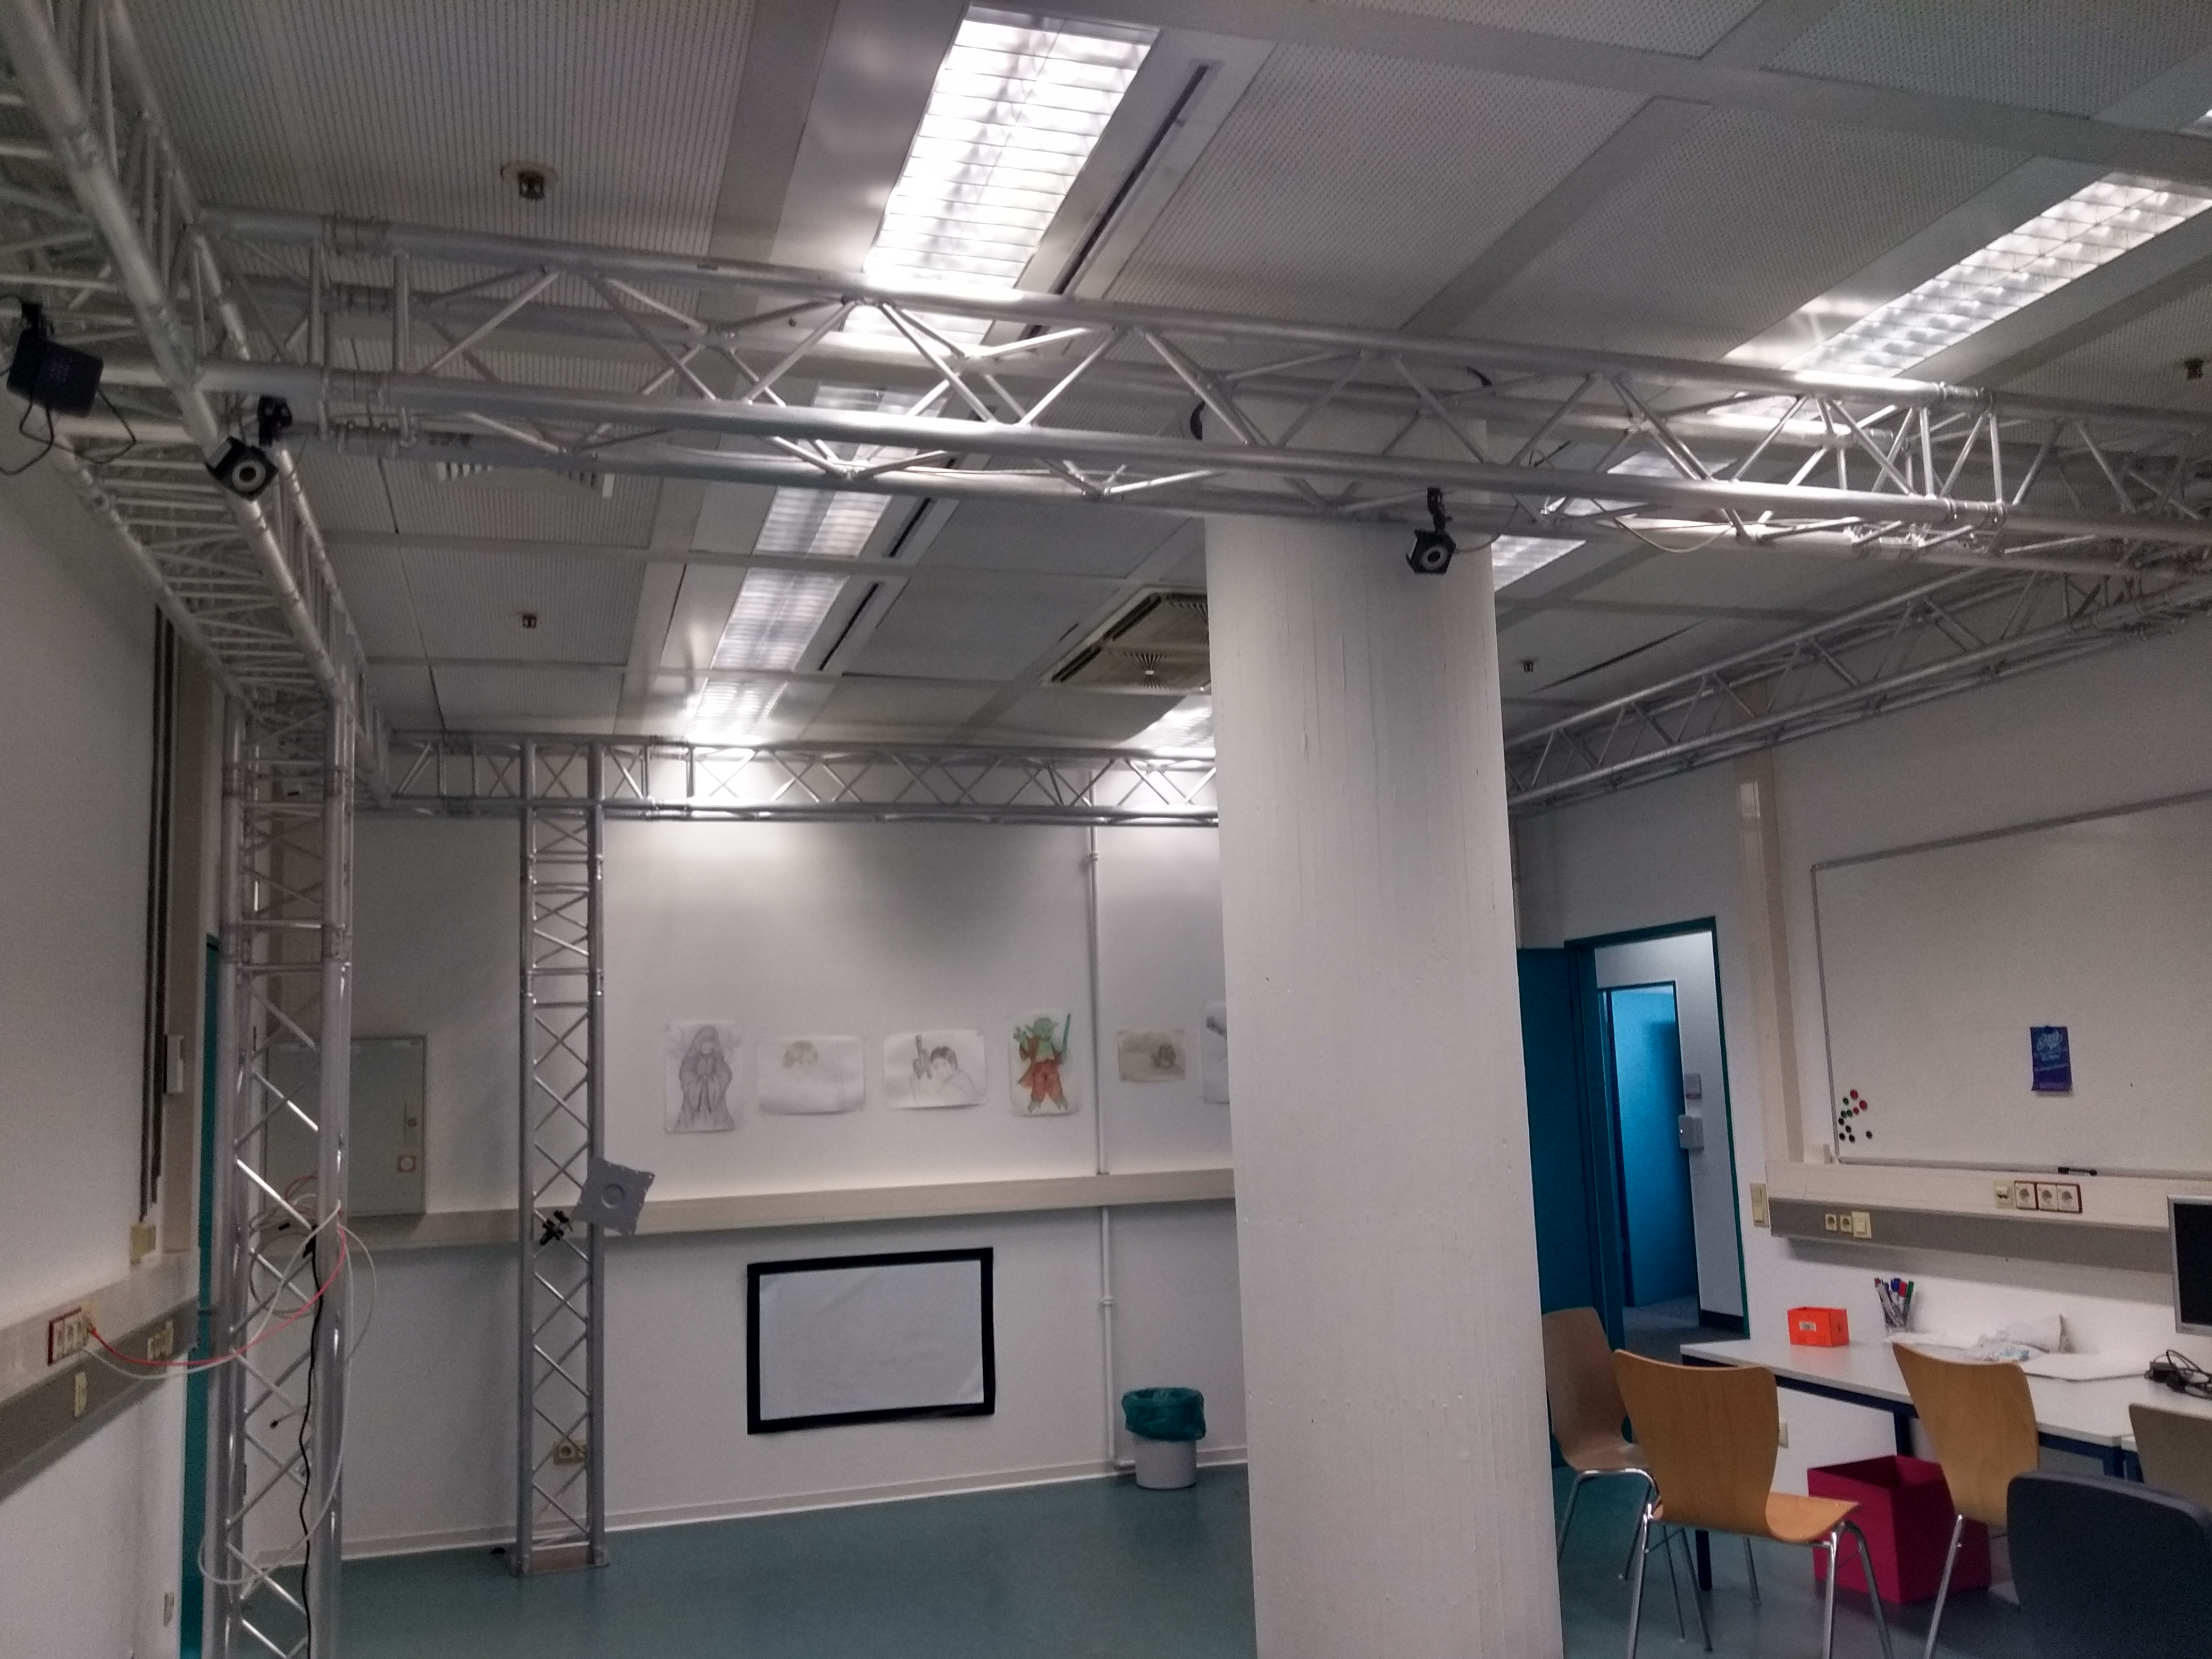
\includegraphics[width=0.755\textwidth]{figures/photo_lab}
        \caption{}
        \label{sfig:lab_photo}
    \end{subfigure}
    \hfill
    \begin{subfigure}{0.49\textwidth}
        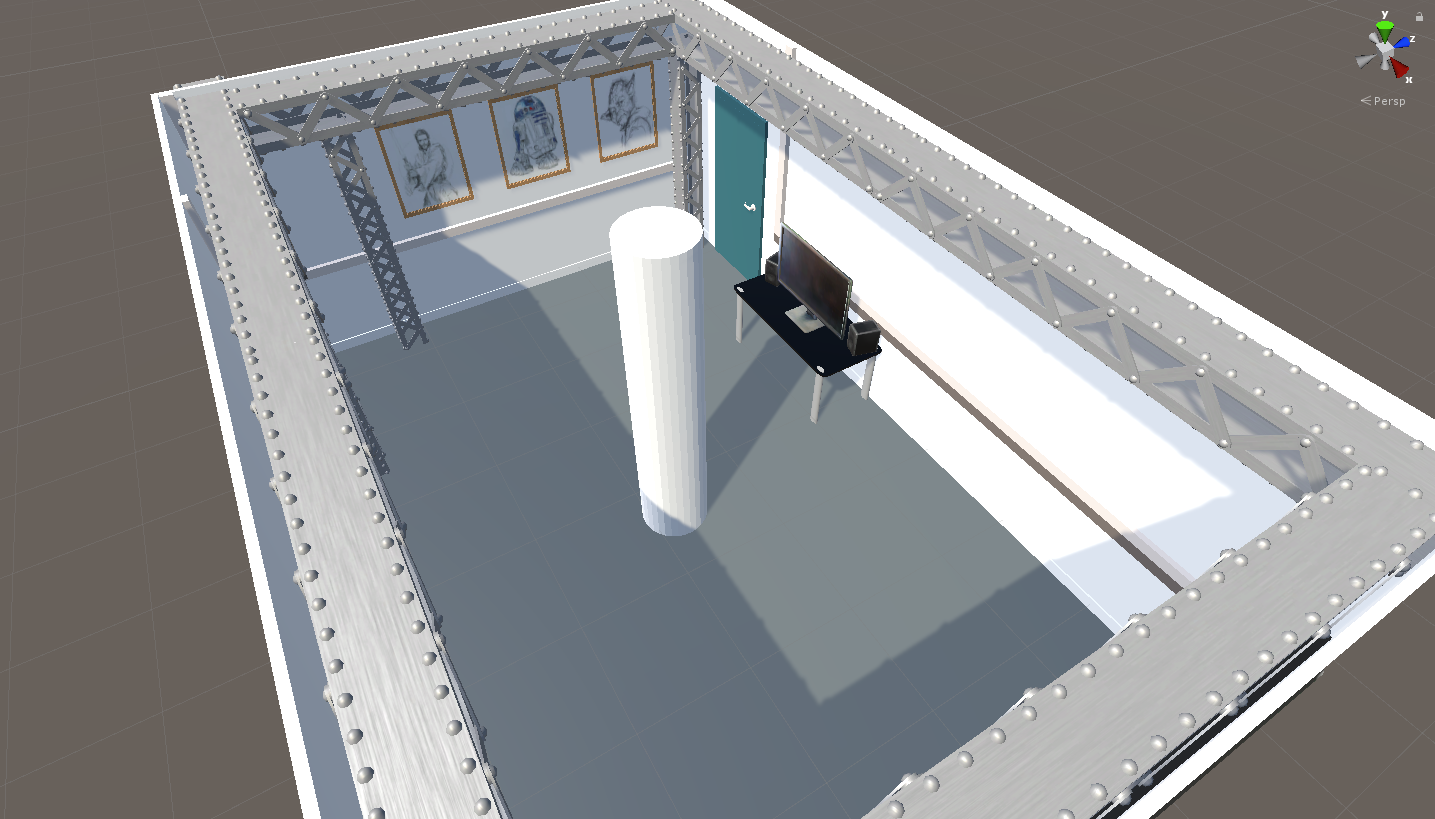
\includegraphics[width=\textwidth]{figures/lab3}
        \caption{}
        \label{sfig:lab_screenshot_1}
    \end{subfigure}

    \vspace{1em}
    \begin{subfigure}{0.49\textwidth}
        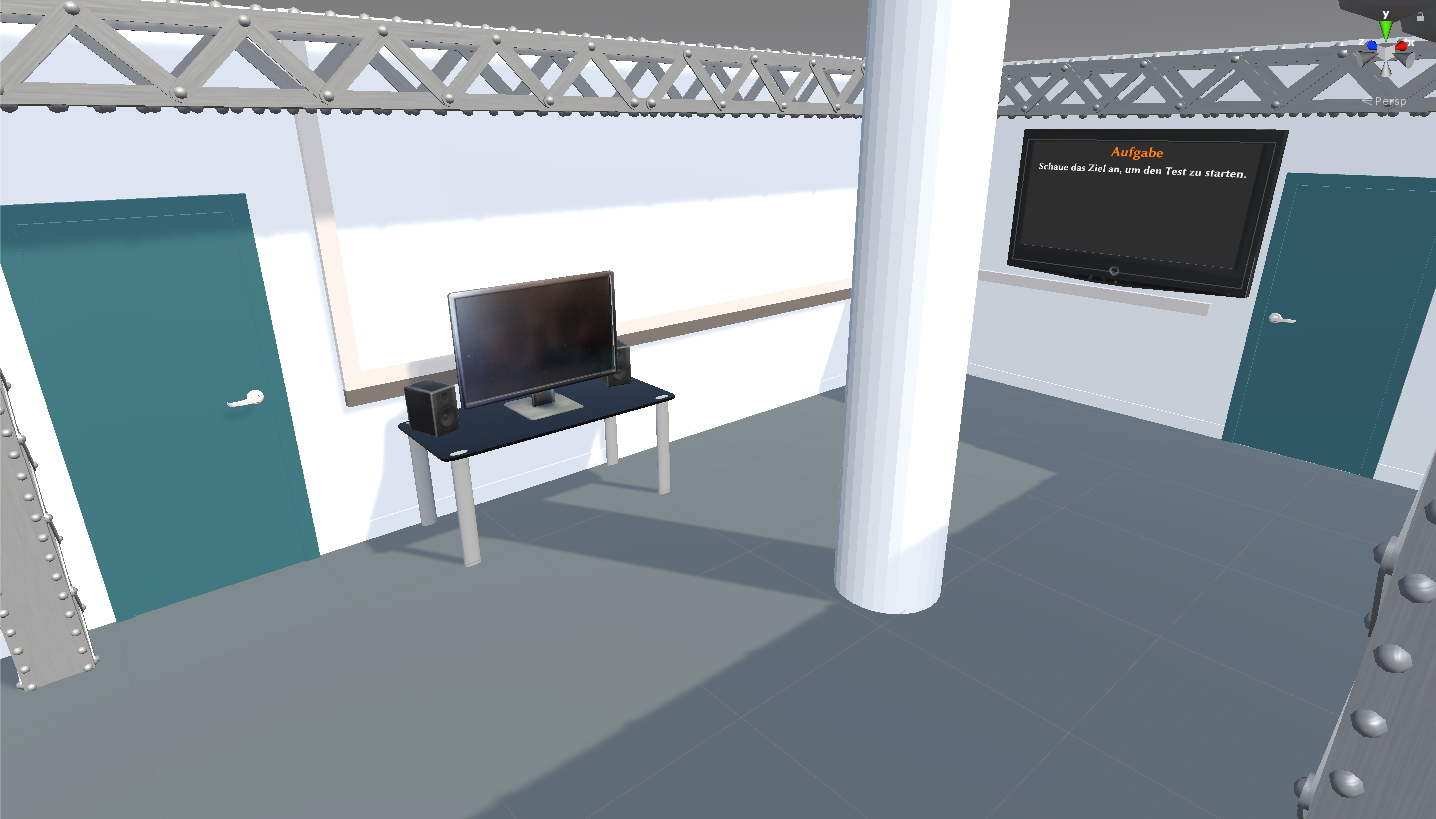
\includegraphics[width=\textwidth]{figures/lab1}
        \caption{}
        \label{sfig:lab_screenshot_2}
    \end{subfigure}
    \hfill
    \begin{subfigure}{0.49\textwidth}
        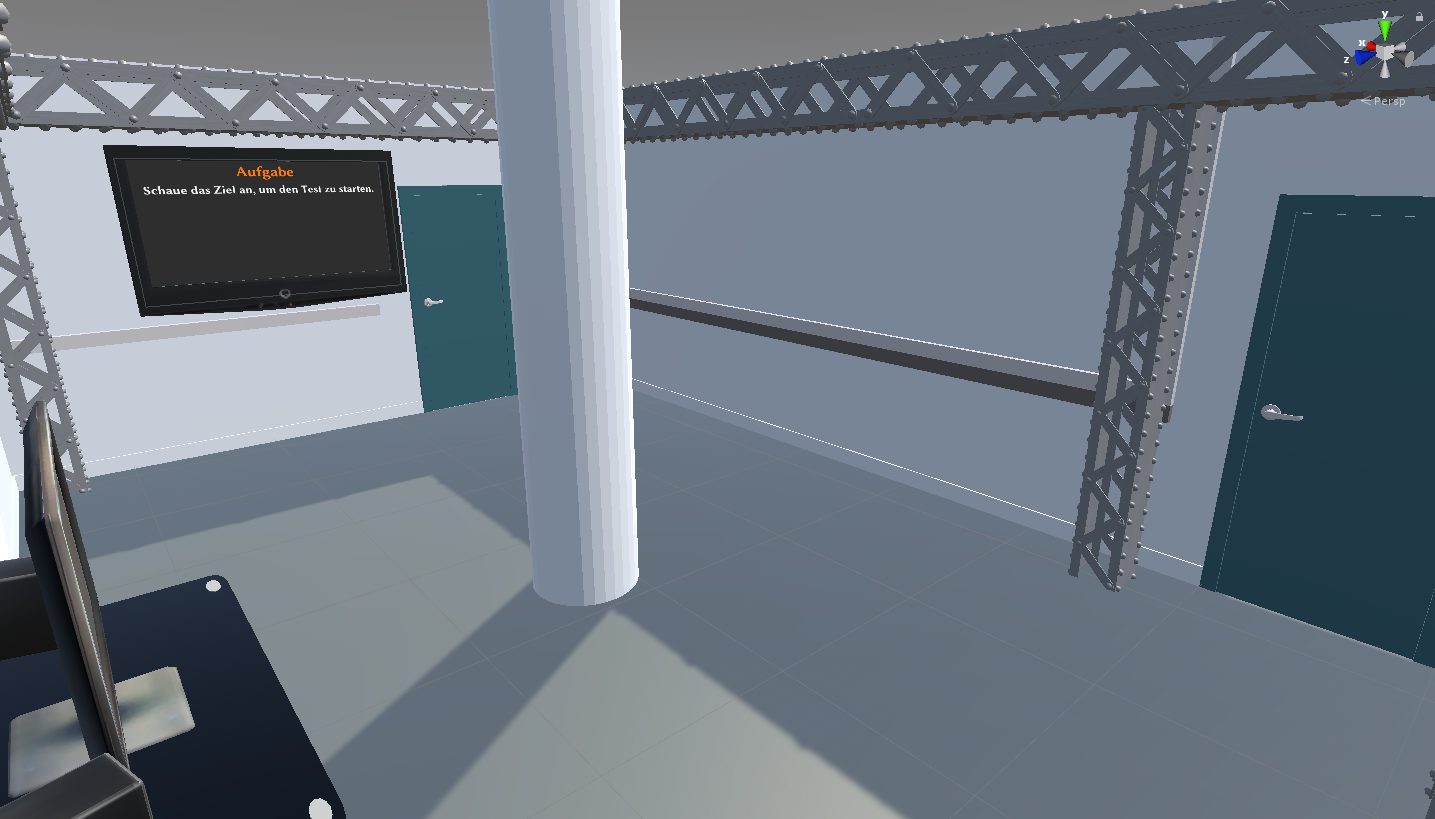
\includegraphics[width=\textwidth]{figures/lab2}
        \caption{}
        \label{sfig:lab_screenshot_3}
    \end{subfigure}
    \caption{Um die Situation der MR-Anwendung in VR nachzubilden, wurde der Laborraum im Maßstab 1:1 modelliert. %
             \subref{sfig:lab_photo} Foto des realen Laborraums. %
             \subref{sfig:lab_screenshot_1}--\subref{sfig:lab_screenshot_3} Screenshots des virtuellen Laborraums in Unity.%
	}
	\label{fig:lab_environment}
\end{figure}

\subsection*{Synchronisation der realen und virtuellen Position}
Damit die virtuelle Umgebung als Ersatz für die reale Umgebung verwendet werden kann muss sichergestellt werden, dass die Rotation des virtuellen Raums der des realen Raums entspricht \emph{und} dass die Position des Nutzers in der virtuellen Welt seiner Position in der realen Welt entspricht.
Der Prototyp muss dafür vorab in zwei Schritten konfiguriert werden:

\paragraph{Erster Schritt:}
Während der Kalibrierung der Vive legt der Nutzer den Spielebereich (die sogenannte \emph{Play Area}) fest.
Dies ist der Bereich, in dem sich keine Hindernisse für den Nutzer befinden und der für die Basisstationen sichtbar ist.
Hierfür zieht der Nutzer mit den Controllern ein Rechteck nach, welches dann als Spielebereich gesetzt wird.

Es wichtig, dass die längere Seite des Rechtecks orthogonal zur Ausgangsrotation des \texttt{Player}-Objekts in Unity verläuft.
Die aktuell getrackte Rotation des HMDs wird relativ zur Ausrichtung der Play Area gemessen.
Da SteamVR automatisch die längeren Seiten der Play Area als Vorder- bzw. Rückseite betrachtet, müssen diese orthogonal zur Blickrichtung des \texttt{Player}-Objekts verlaufen.
Im Fall des entwickelten Prototypen bedeutet dies, dass die Vorderseite der Play Area parallel zu der Wand des Labors verlaufen muss, an der sich die Eingangstür und Tische befinden (siehe \autoref{fig:lab_environment}).
Die korrekte Kalibrierung der Play Area wird in \autoref{fig:ve_setup_correct} skizziert.

Wenn bei der Kalibrierung der Play Area eine andere Ausrichtung gewählt wird, als die Ausgangsrotation des \texttt{Player}-Objekts, weicht die virtuelle Rotation des Nutzers von der realen Rotation im Bezug zum Raum ab.
Effektiv hätte die virtuelle Umgebung dann eine andere Ausrichtung als die reale Umgebung.
Die falsche Kalibrierung wird in \autoref{fig:ve_setup_wrong} dargestellt.

Ginge es nur um den visuellen Reiz in der virtuellen Umgebung, würde der Nutzer diese Abweichung lediglich beim Aufsetzen des HMDs bemerken (da dann der virtuelle Raum anders rotiert wäre als der reale).
Wenn aber zum Beispiel der Tastsinn eine Rolle spielt, dann ist eine korrekte Ausrichtung des virtuellen Raums sinnvoll.
Da in dem entwickelten Prototyp nicht ausgeschlossen ist, dass der Nutzer die Play Area verlässt und beispielsweise die Säule oder Wände mit den Händen berührt, ist es für die Immersion von Vorteil, wenn das Berühren der virtuellen Objekte mit den taktilen Reizen der realen Objekte verknüpft wird.
Weiterhin wird durch die korrekte Ausrichtung die Messung des Abweichungsfehlers beim Zeigen auf Objekte erleichtert, was detailliert in \autoref{chap:evaluation} beschrieben wird.

\begin{figure}
    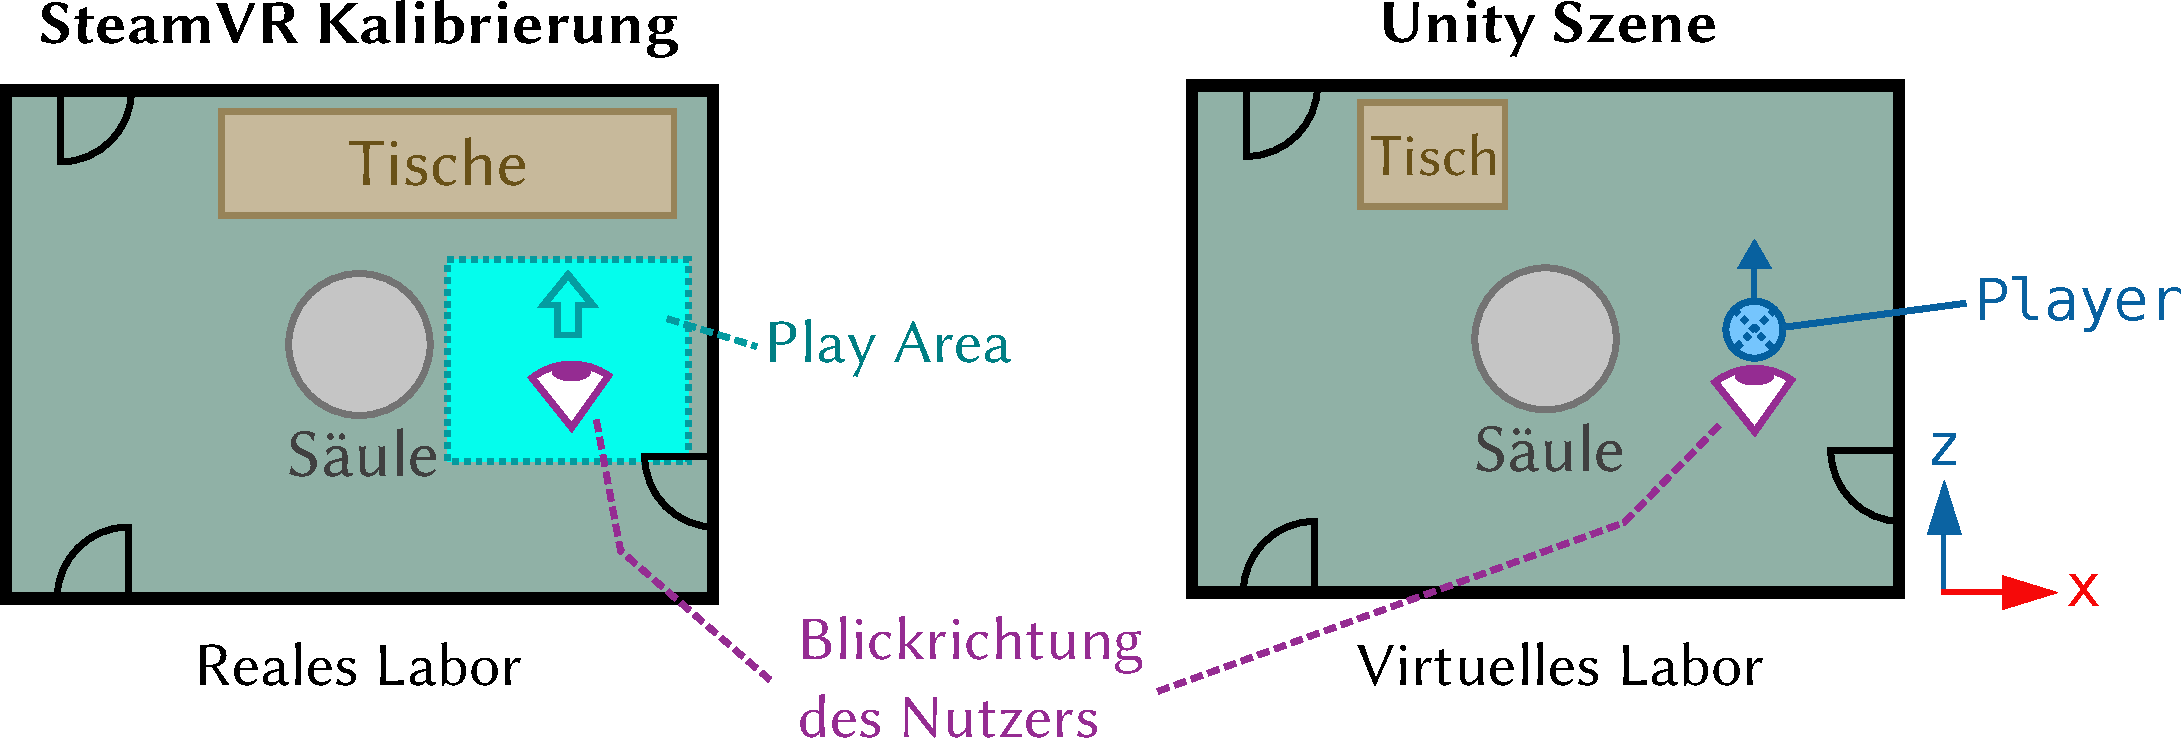
\includegraphics[width=\textwidth]{figures/environment_setup_correct}
    \caption{Die Play Area hat die gleiche Ausrichtung wie das \texttt{Player}-Objekt in der Grundrotation (entlang z-Achse). %
    Die Rotation des Nutzers in der realen und virtuellen Welt stimmt überein.}
    \label{fig:ve_setup_correct}
\end{figure}

\begin{figure}
    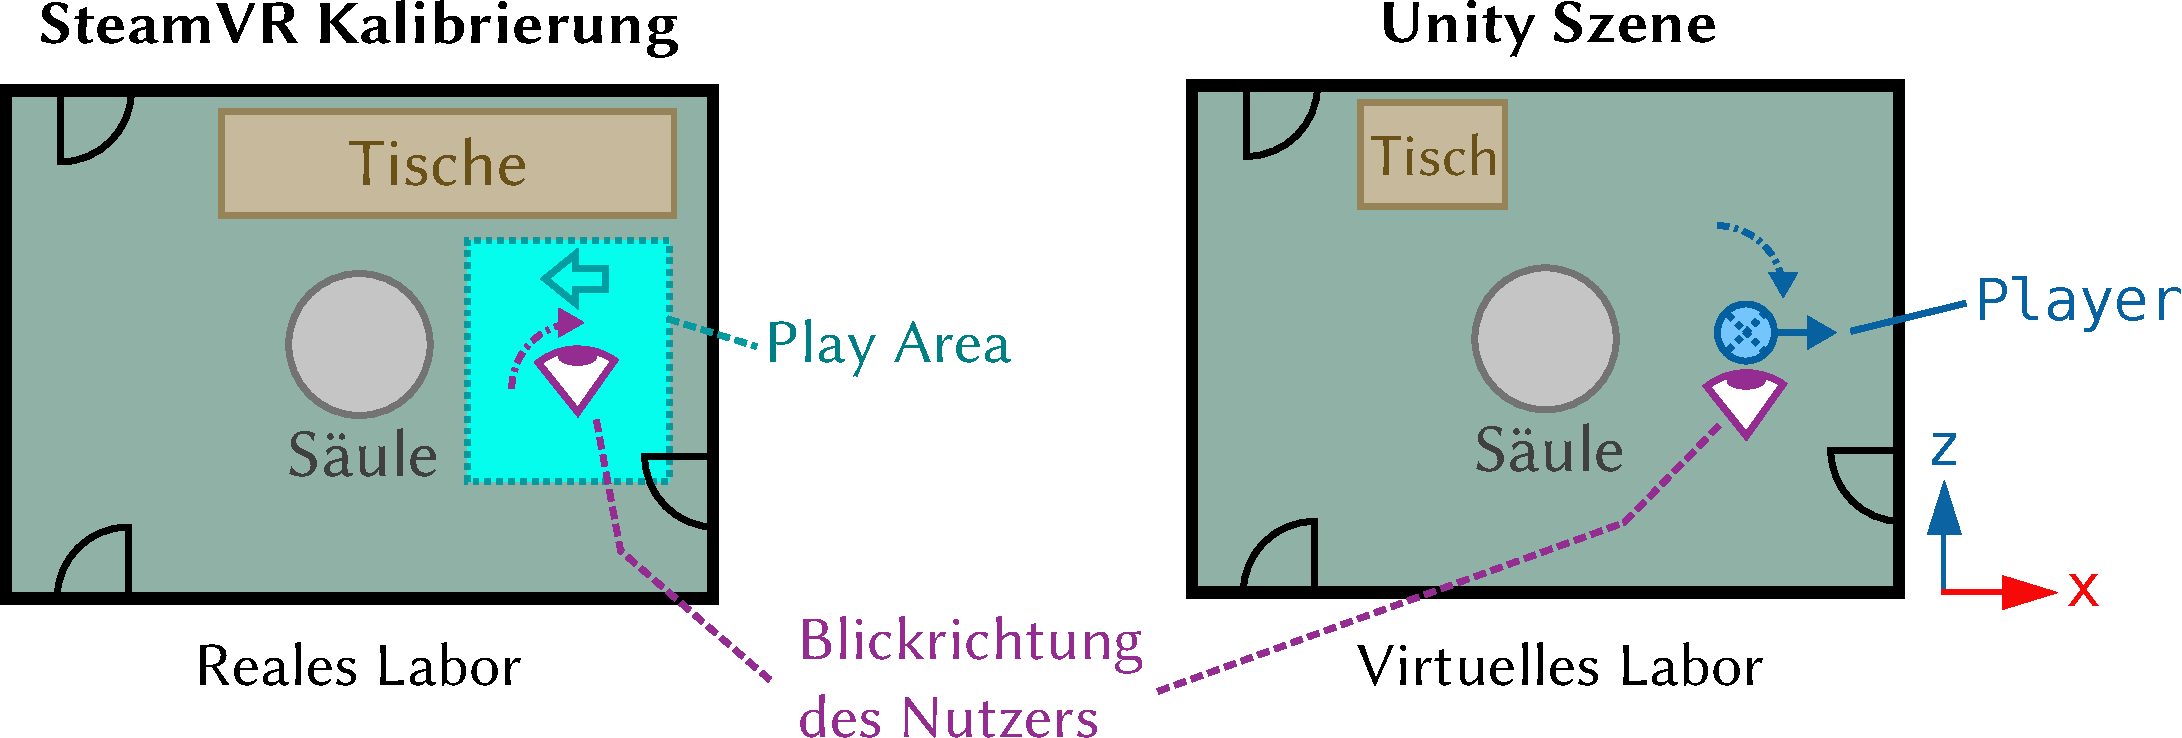
\includegraphics[width=\textwidth]{figures/environment_setup_wrong}
    \caption{Die Play Area hat \emph{nicht} die gleiche Ausrichtung wie das \texttt{Player}-Objekt in der Grundrotation. %
        Der Nutzer hat einen Rotationsoffset (hier \ang[detect-weight=true]{90}), wodurch für den Nutzer effektiv die Räume unterschiedlich rotiert wirken.}
    \label{fig:ve_setup_wrong}
\end{figure}

\paragraph{Zweiter Schritt:}
Neben der Orientierung des Nutzers muss die Position des virtuellen Raums angepasst werden, wenn dieser die reale Umgebung bestmöglich überlagern soll.
Dies resultiert (wie bei der Rotation) aus der Tatsache, dass die getrackte Position des HMDs im Bezug zur Play Area gemessen wird, welche sich durch den Kalibrierungsvorgang von SteamVR ändern kann.
Um neue Position des virtuellen Raums zu bestimmen wird für den Prototypen wie folgt vorgegangen:

Der Prototyp wird mit seiner Ausgangsposition im Unity Editor ausgeführt.
Die Ecke \enquote{links unten} aus Vogelperspektive des virtuellen Labors befindet sich an der Unity-Welt-Koordinate $(0, 0, 0)$.
Die Controller, welche im HMD durch 3D-Modelle visualisiert sind, werden in den Ecken des virtuellen Raums platziert.
Dabei wird darauf geachtet, dass sie von den Basisstationen weiterhin erkannt werden.
Nun wird im realen Labor die Entfernung von den Controllern zu den entsprechenden Ecken des Raums gemessen, was der Abweichung der virtuellen Welt entspricht.
Die Entfernungen werden gemittelt.
Der resultierende Offset wird dann im Unity Editor verwendet, um das virtuelle Labor zu verschieben.
Dieser Offset ist nun solange gültig, bis die Play Area neu kalibriert wird.

Wie auch schon bei der Rotation ist diese Angleichung erst dann für die Nutzer bemerkbar, wenn sie versuchen physische Objekte wie Wände oder die Säule zu berühren.
Würde die Verschiebung des Raums nicht durchgeführt werden, könnten Nutzer mit den Controllern durch die virtuellen Objekte hindurch greifen oder sie würden auf physische Barrieren stoßen, obwohl die virtuellen Objekte noch weiter entfernt sind.

Nach diesen beiden Schritten kann der virtuelle Raum als Ersatz für die reale Umgebung verwendet werden, die in einer MR-Anwendung ohne vorheriges Modellieren verfügbar wäre.

\section{Das Megamap-GameObject}
\begin{figure}[t]
    \centering
    \imagebox{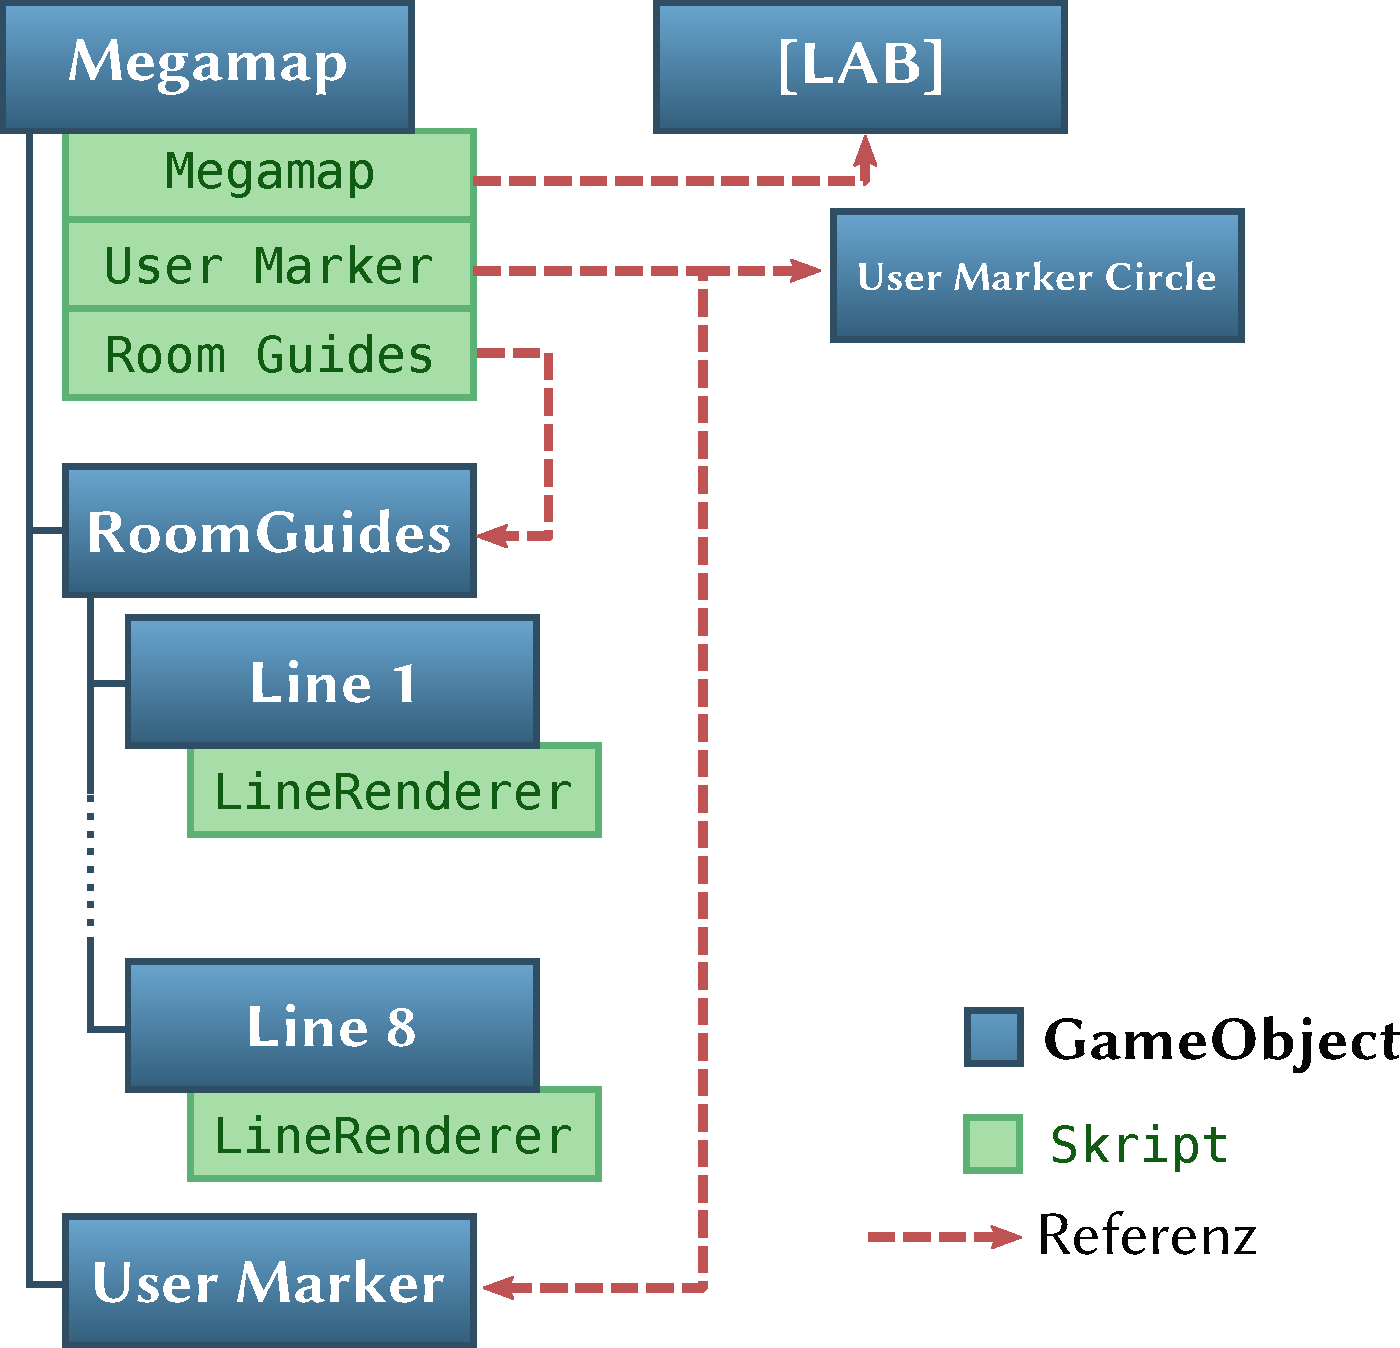
\includegraphics[height=8.5cm]{figures/unity_megamap_object}}
    \caption{Übersicht des Megamap-GameObjects.}
    \label{fig:unity_megamap_object}
\end{figure}

Eine grundlegende Implementierung des in \autoref{chap:concept} vorgestellten Megamap-Konzepts wird im Megamap-GameObject realisiert.
Eine strukturelle Übersicht des Objekts wird in \autoref{fig:unity_megamap_object} gegeben.
Das Objekt setzt sich aus drei Teilen zusammen, die jeweils durch eigene Komponenten repräsentiert werden:

Das Skript \textbf{\texttt{Megamap}} bietet allgemeine Einstellungsmöglichkeiten zur Darstellung der Megamap.
Es lassen sich z.B. die Skalierung oder die Höhe vom Boden ändern.
Weiterhin bietet das Skript die Methoden \texttt{Show()} und \texttt{Hide()}, mit denen die Karte angezeigt bzw. ausgeblendet werden kann.
Falls dabei das Feld \texttt{useAnimation} auf \texttt{true} gesetzt ist, wird die Karte beim Anzeigen von einer 1:1 Raumgröße auf die eingestellte Skalierung herunterskaliert (beim Ausblenden analog ein Hochskalieren).
Die Megamap wird standardmäßig Nutzer-zentriert platziert.
Das bedeutet, dass der Nutzer sowohl in der realen Welt als auch auf der Karte die gleiche Position einnimmt.
Hierfür wird die virtuelle Umgebung referenziert und der Abstand vom HMD zum Ursprung des Labor-Modells ermittelt.
Dieser Abstand wird dann wie die Megamap skaliert und die Karte wird um den skalierten Abstand verschoben.
Sowohl die Animation als auch die Zentrierung auf den Nutzer sollen es ihm erleichtern, seine eigene Position auf der Karte zu finden.
Außerdem soll hierdurch der Bezug vom Laborraum auf der Karte zum umgebenden Laborraum hervorgehoben werden.

Der zweite Teil des Megamap-Objekts, das \textbf{\texttt{User Marker}}-Skript, dient ebenfalls der Orientierung für den Nutzer.
Analog zu Kartenanwendungen wie Google Maps befindet sich ein Marker auf der Megamap, welcher die aktuelle Position des Nutzers anzeigt.
Da es sich bei der Megamap um eine dreidimensionale Karte handelt wird hier ein Zylinder in Form ähnlich eines Pucks benutzt (siehe \autoref{fig:user_marker}).
Mittels eines transparenten Kreissegments wird außerdem die aktuelle Rotation des Nutzers verdeutlicht.
Um den Bezug vom Marker auf der Karte zur Umgebung zu verstärken ist auch in dieser ein Kreis platziert, welcher auf dem Nutzer zentriert ist.

\section{Erstellung der Indoor-Karten}
\label{sec:indoor_maps}

\section{Interaktion mittels virtuellem Laserpointer}

\section{Automatisierung durch georeferenzierte Gebäudedaten}

\subsection{WRLD SDK}

Das \emph{WRLD SDK} (fortan \enquote{WRLD}) ein Framework, um interaktive 3D-Karten zu erstellen und anzuzeigen.
Es unterstützt mehrere Plattformen und bietet zudem ein Plugin für Unity an.
WRLD bezieht dabei seine Kartendaten von \emph{OpenSteetMap} sowie diversen proprietären Anbietern \parencite{WRLD2018}.
Die Daten werden aufbereitet und Nutzern über WRLDs eigene Server zur Verfügung gestellt.
Eine AR-Beispielanwendung ist in \autoref{fig:wrld_ar} zu sehen.
\begin{figure}
    \centering
    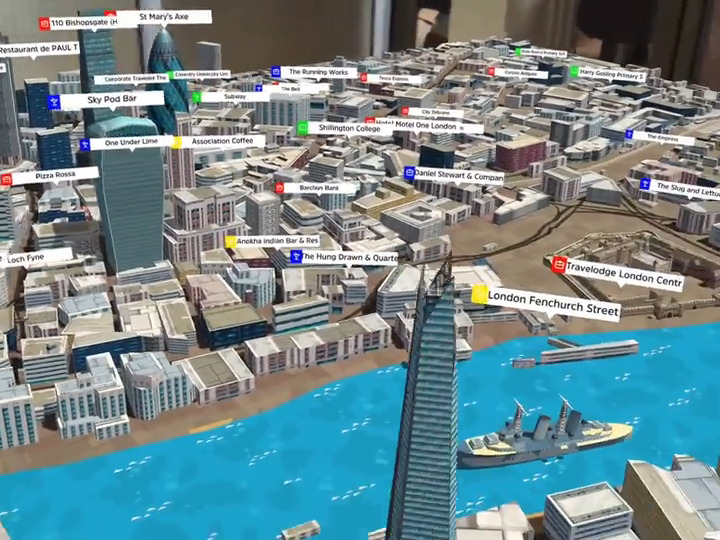
\includegraphics[width=\textwidth]{figures/wrld_ar-web-11}
    \caption{AR-Anwendung von WRLD, welche eine 3D-Ansicht von London auf einem Tisch platziert. \quelle{\cite{WRLD2018b}}}
    \label{fig:wrld_ar}
\end{figure}

Das Besondere an WRLD ist, dass es eine Funktion zur Einbettung von Indoor-Karten von Gebäuden bietet.
Hierzu können Entwickler georeferenzierte Lagepläne auf die WRLD-Server hochladen und für das gewünschte Gebäude registrieren.
Danach sind die Indoor-Karten für die Gebäude öffentlich für alle Nutzer von WRLD zugänglich.
Zudem können die Indoor-Karten mit Einrichtungsgegenständen versehen werden, um die Karten natürlicher aussehen zu lassen.
\autoref{fig:wrld_indoor} zeigt die Interaktion mit WRLDs Indoor-Karten.
In der Karten-3D-Ansicht kann über einen Button das Gebäude betreten werden (falls eine Indoor-Karte für das Gebäude vorhanden ist).
Über einen Slider kann das anzuzeigende Stockwerk ausgewählt werden.
Dabei werden alle Stockwerke des Gebäudes mit einer Animation aufgefächert und mit dem Slider durchlaufen.
Schließlich wird das ausgewählte Stockwerk angezeigt.
Alle Stockwerke oberhalb des Aktuellen werden ausgeblendet, die darunterliegenden werden durch das Aktuelle überdeckt.
\begin{figure}
    \begin{subfigure}{0.49\textwidth}
        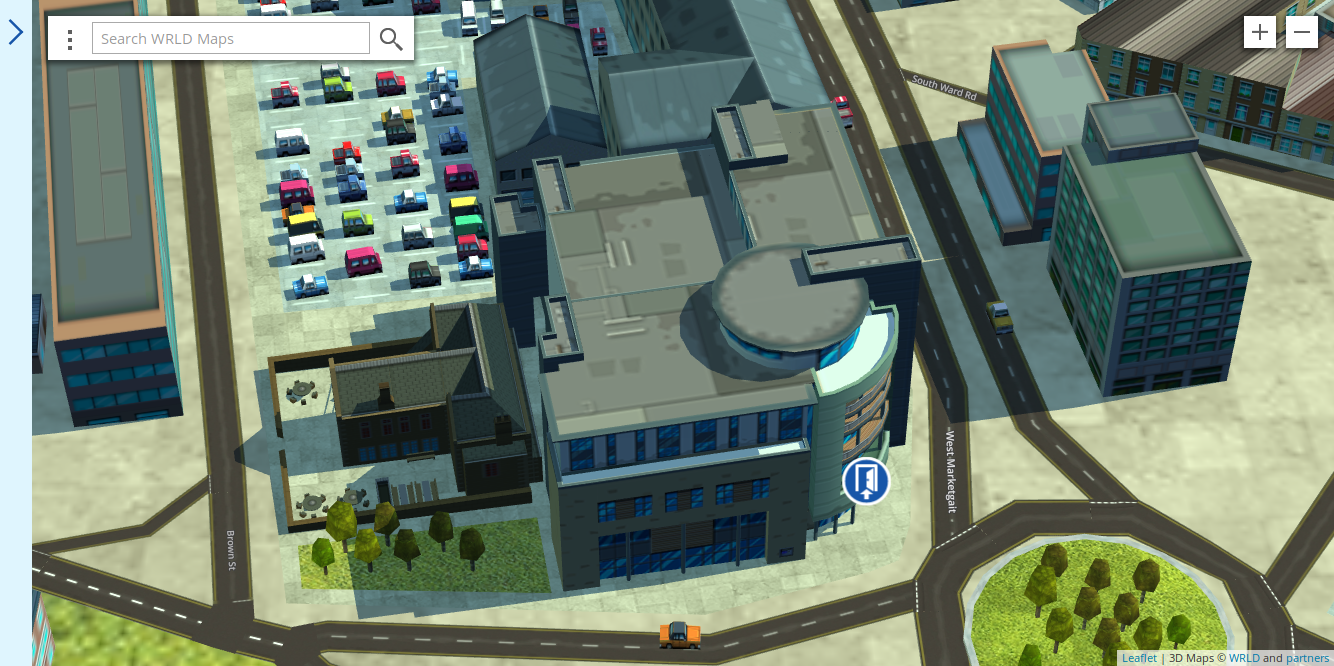
\includegraphics[width=\textwidth]{figures/wrdl_outdoor.png}
        \caption{}
        \label{sfig:wrld_outdoor}
    \end{subfigure}
    \hfill
    \begin{subfigure}{0.49\textwidth}
        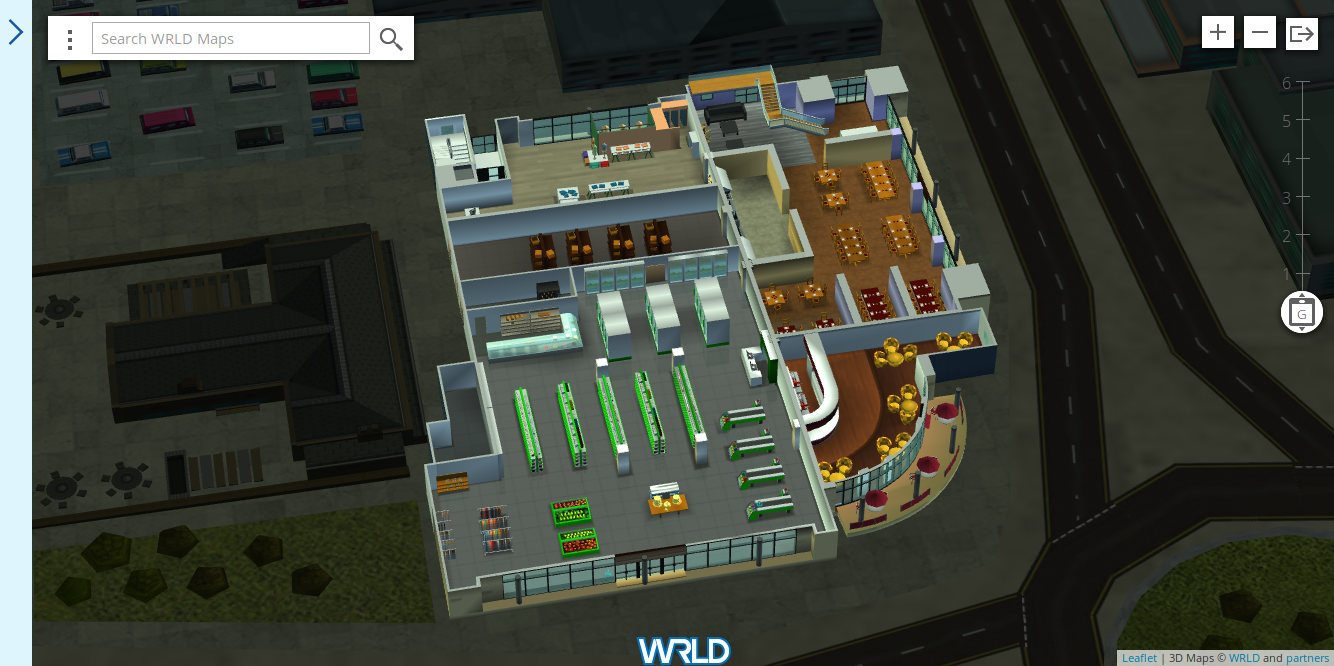
\includegraphics[width=\textwidth]{figures/wrdl_indoor_g.png}
        \caption{}
        \label{sfig:wrld_indoor_g}
    \end{subfigure}
    \newline
    \begin{subfigure}{0.49\textwidth}
        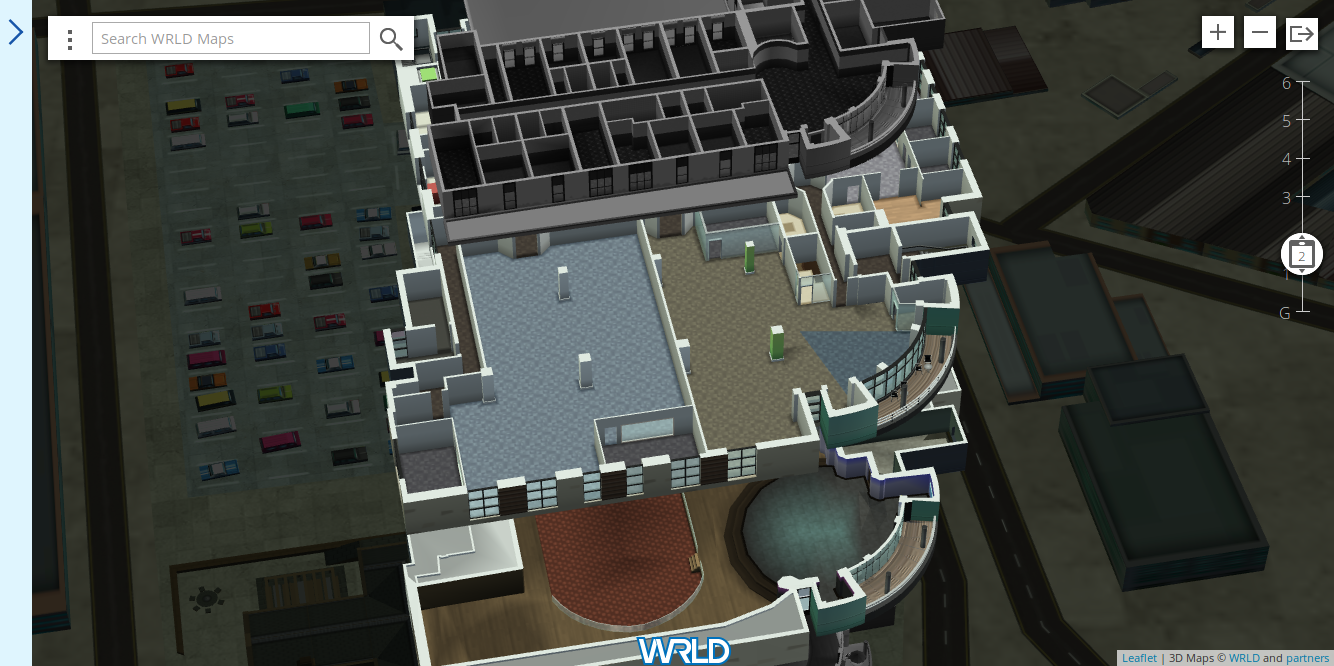
\includegraphics[width=\textwidth]{figures/wrdl_indoor_transition.png}
        \caption{}
        \label{sfig:wrld_indoor_transition}
    \end{subfigure}
    \hfill
    \begin{subfigure}{0.49\textwidth}
        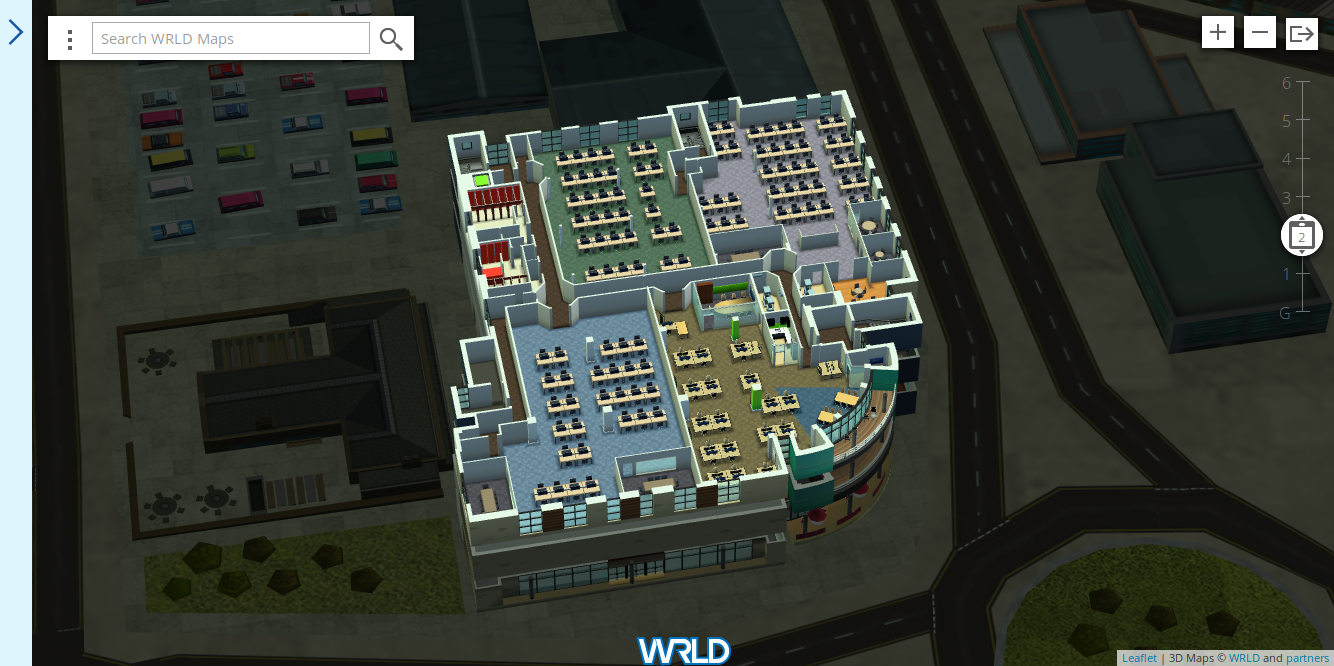
\includegraphics[width=\textwidth]{figures/wrdl_indoor_2.png}
        \caption{}
        \label{sfig:wrld_indoor_2}
    \end{subfigure}
    \caption{Indoor-Funktionalität von WRLD.\@ %
        \subref{sfig:wrld_outdoor} Das Gebäude ist von außen sichtbar. %
        Über einen Button kann das Gebäude betreten werden. %
        \subref{sfig:wrld_indoor_g} Die Innenansicht des Gebäudes mitsamt Einrichtung wird angezeigt. %
        \subref{sfig:wrld_indoor_transition} Über einen Slider können die Stockwerke gewechselt werden. %
        \subref{sfig:wrld_indoor_2} Untenliegende Stockwerke werden vom aktuellen Stockwerk verdeckt.%
    }
    \label{fig:wrld_indoor}
\end{figure}

Für das Ziel dieser Arbeit (die Implementierung einer Indoor-Megamap im Stil von TCTD) wäre WRLD durch seine Indoor-Funktionalität eine ideale Grundlage.
Allerdings hat das SDK einen Nachteil, welches den Einsatz für diese Arbeit unmöglich macht.
Um eine Indoor-Karte in das SDK einzubinden, muss diese für das entsprechende Gebäude auf die WRDL-Server hochgeladen werden.
Im Fall dieser Arbeit wäre das eine Indoor-Karte für das MZH der Universität Bremen.
WRLDs Kartenabdeckung für Deutschland ist jedoch nur teilweise vorhanden; die Daten für Bremen fehlen komplett.
Das MZH steht somit beim Upload der Karte nicht zur Verfügung.
Die Recherche des Verfassers dieser Arbeit ergab keine Möglichkeit, den Upload auf die Server durch eine Offline-Nutzung des SDKs zu umgehen.
Daher muss bei der Implementierung der Megamap auf WRLD verzichtet werden.
Die Art der Darstellung und Integration der Indoor-Karte in die Umgebung sowie der Wechsel zwischen den Stockwerken dient jedoch als Inspiration für die Implementierung einer eigenen Lösung.

\subsection{Mapbox SDK}
% TODO: Grafik für nicht funktionierende Pipeline?
Als Alternative zu WRLD bietet sich das Mapbox SDK an.
Mapbox bietet Schnittstellen zur Anzeige von Karten, Routennavigation sowie Visualisierung von kartenbasierten Daten.
Ähnlich wie bei Google Maps werden die Karten in \emph{\enquote{Tiles}} geliefert.
Mapbox bietet sowohl Raster-Tiles (Satellitenbilder) als auch Vektor-Tiles (vektorbasierte Straßen- und Gebäudeumrisse) an.
Mapbox bezieht seine Daten über unterschiedliche Provider, einschließlich OpenStreetMap \autocite{Mapbox2018}.
Über ein Plugin lässt sich Mapbox als Paket in Unity einbinden.
Mit dem \unity{AbstractMap}-Prefab kann auf die Hauptfunktionalität von Mapbox zugegriffen werden.

Mapbox erlaubt wie WRLD eine 3D-Ansicht der Karte, inklusive Gebäude.
Sofern die OpenStreetMap-Daten Informationen über die Beschaffenheit der Gebäude liefern, wie z.B. die Höhe, können diese Daten für eine 3D-Visualisierung mit Mapbox ausgelesen werden.
Dazu wird als Grundlage ein Vektor-Tile der Umgebung verwendet.
Für die Umrisse der Gebäude werden dann Polygone generiert und entsprechend der Höhe extrudiert.
\autoref{fig:mapbox_unity_uni_bremen} zeigt eine 3D-Ansicht des zentralen Gebäudekomplexes der Universität Bremen.
Die hier verwendeten Gebäudedaten stammen alle von OpenStreetMap.
Über weitere Einstellungen ließen sich weiterhin die farbliche Darstellung der Gebäude anpassen.
Die Darstellung weist allerdings Probleme auf, auf die später näher eingegangen wird.

\begin{figure}
    \centering
    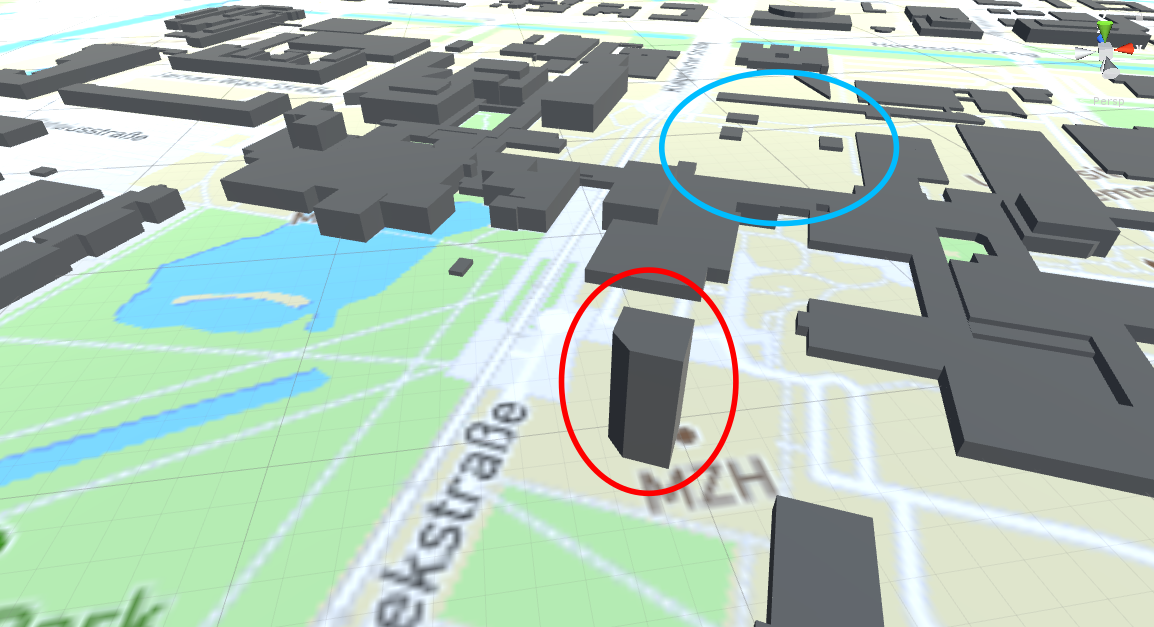
\includegraphics[width=\textwidth]{figures/mapbox_unity_uni_bremen_markings}
    \caption{3D-Darstellung der Universität Bremen via Mapbox und Unity. %
    Die Gebäudedaten bezieht Mapbox von OpenStreetMap. %
    \textcolor{red}{Rot:} Fehlende Geometrie beim MZH.\@ %
    \textcolor[HTML]{00bdff}{Blau:} Fehlende Geometrie beim GW2. %
    (\textit{Farbversion dieses Dokuments wird empfohlen.})}
    \label{fig:mapbox_unity_uni_bremen}
\end{figure}

Anders als bei WRLD gibt es bei Mapbox keine \emph{explizite} Unterstützung von Indoor-Karten.
Jedoch lassen sich diese über einen Umweg einbinden, wie \textcites{Mapbox2018b}{Pavani2018}{Clarke2017} präsentieren.
Zuerst muss ein georeferenzierter Lageplan des Gebäudes erstellt werden.
Dies kann z.B. mit der Software \emph{QGIS} umgesetzt werden.
Für diese Arbeit wurde zunächst die Ebene 5 des MZH an der Universität Bremen basierend auf dem Lageplan des Gebäudes in QGIS georeferenziert.
Beim Georeferenzieren werden die Räume und Wände durch Polygone dargestellt.
Jeder Vertex besitzt neben seiner x- und y-Position eine weitere Koordinate in Bezug auf ein geographisches Koordinaten-Referenz-System (KRS).
% TODO: Mapbox' KRS einfügen
Mapbox verwendet hier das \texttt{???} KRS, wodurch jeder Vertex einen Breitengrad (\emph{\enquote{Latitude}}) im Bereich \ang{-90} bis \ang{90} und einen Längengrad (\emph{\enquote{Longitude}}) im Bereich \ang{-180} bis \ang{180} erhält.
Der \emph{Breitengrad} wird von Norden nach Süden gemessen, wobei der Äquator den Breitengrad \ang{0} hat.
Grade nördlich vom Äquator sind daher positiv, Grade südlich vom Äquator sind negativ.
Der \emph{Längengrad} wird von Osten nach Westen gemessen.
Dabei hat der \emph{Nullmeridian} (\emph{\enquote{Prime Meridian}}; der Halbkreis vom Nordpol durch Greenwich in England bis zum Südpol) den Längengrad \ang{0}.
Grade östlich vom Nullmeridian sind positiv, Grade westlich vom Nullmeridian sind negativ \autocite{ESRIInc2018}.
Jeder Punkt auf der Erdoberfläche kann durch Angabe des Breiten- und Längengrads referenziert werden.
\autoref{fig:latlong_from_globe_center} zeigt dies graphisch.
Als Beispiel hat der Mittelpunkt des MZH in etwa den Breitengrad \ang{53,10668} und den Längengrad \ang{8,85238}.

\begin{figure}
    \centering
    \imagebox{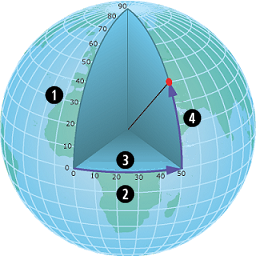
\includegraphics[width=0.35\textwidth]{figures/latlong_from_globe_center}}
    \caption{(1) Breitengrad (2) Längengrad (3) \ang[detect-weight=true]{50} östlich (4) \ang[detect-weight=true]{40} nördlich. \quelle{\cite{ESRIInc2018}}}
    \label{fig:latlong_from_globe_center}
\end{figure}

Durch das Georeferenzieren können die Räume eindeutig auf einer Karte platziert werden.
Der georeferenzierte Lageplan der Ebene 5 des MZH ist in \autoref{fig:qgis_mzh_e5} zu sehen.
Die Räume werden durch die blauen Polygone dargestellt und die Wände durch die grauen.

\begin{figure}
    \centering
    \imagebox{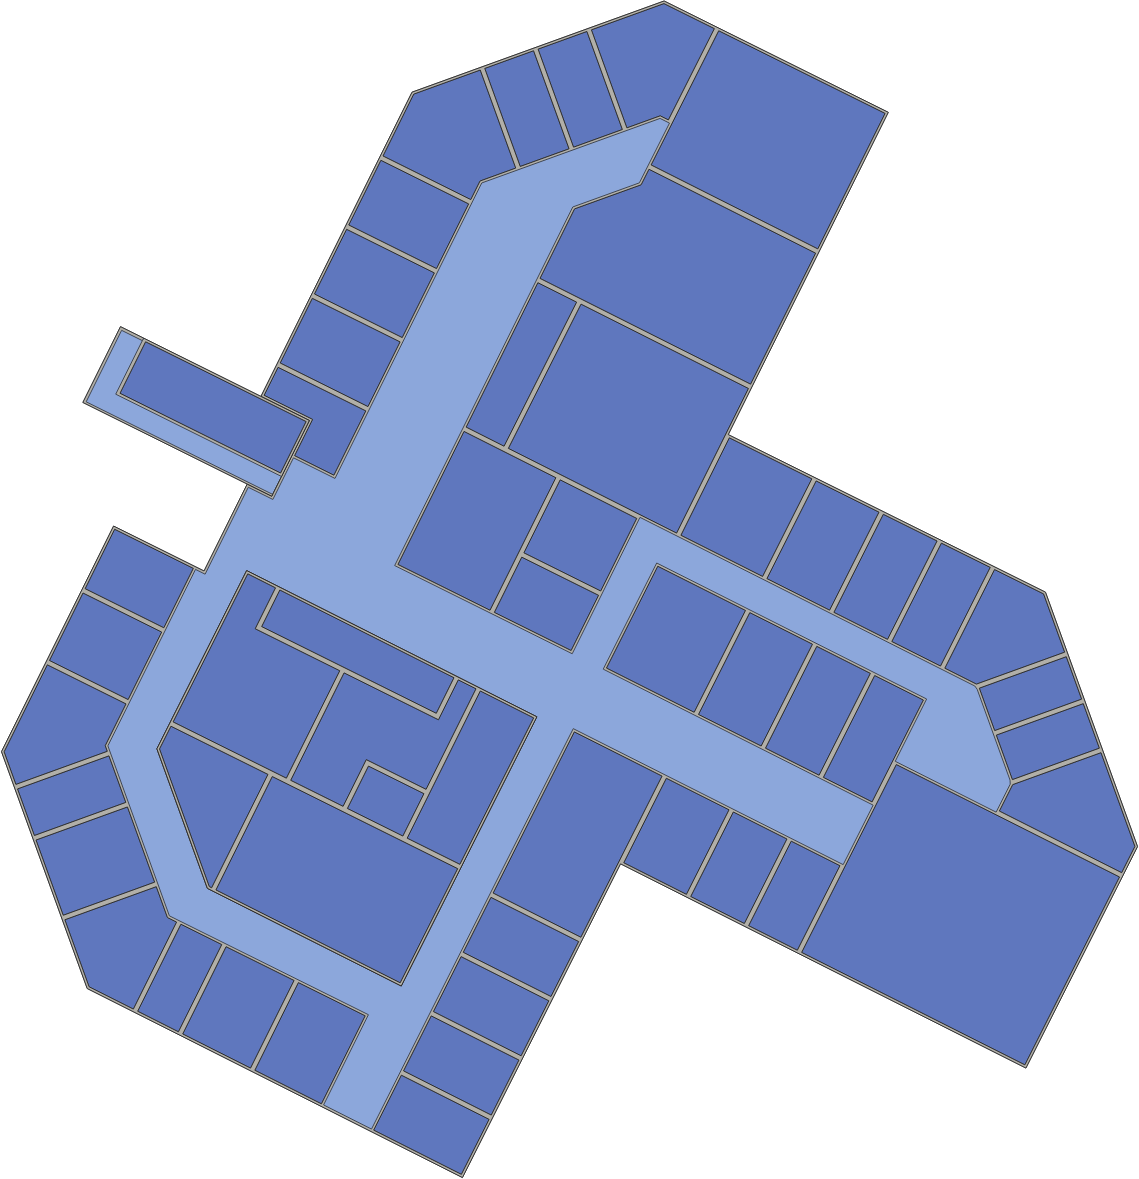
\includegraphics[width=0.3\textwidth]{figures/qgis_mzh_e5}}
    \caption{Georeferenzierter Lageplan der Ebene 5 des MZH in QGIS.\@ %
    Die blauen Features sind vom Typ \texttt{room}, die grauen vom Typ \texttt{wall}.}
    \label{fig:qgis_mzh_e5}
\end{figure}

Theoretisch ließen sich die Wände anstatt durch Polygone auch durch Linien-Primitive darstellen.
Dies führt bei der 3D-Visualisierung von Mapbox zu Problemen bei der Darstellung von Ecken, wie \autoref{fig:mapbox_wand_ecke_problem} zeigt.
Mapbox generiert für die Linien-Wände Meshes mit einer gewissen Dicke.
Die generierten Meshes werden an Eckpunkten jedoch nicht automatisch verbunden.
Das heißt, dass weitere Ecken entstehen, was nicht der gewünschten Geometrie entspricht.
Das Modellieren der Wände durch Polygone erlaubt mehr Kontrolle über das Aussehen des generierten Meshes.

\begin{figure}
    \centering
    \imagebox{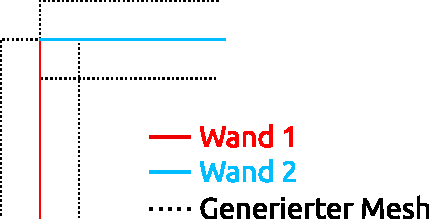
\includegraphics[width=0.6\textwidth]{figures/mapbox_wand_ecke_problem}}
    \vspace{2em}
    \caption{Wenn Wände durch Linien-Primitive repräsentiert werden, generiert Mapbox Meshes, die nicht automatisch verbunden werden.}
    \label{fig:mapbox_wand_ecke_problem}
\end{figure}

Durch das Hochladen auf die Mapbox-Server wird der Lageplan in ein Vektor-Tileset konvertiert.
Auf dieses kann mit dem Unity-Plugin zugegriffen werden.
\autoref{fig:mapbox_unity_mzh_e5_z15} zeigt die 3D-Darstellung des zuvor erstellten Lageplans.
Dabei werden nur Polygon-Features mit dem Attribut \texttt{type = wall} gerendert (das Attribut wird in QGIS gesetzt).
Als Höhe wurde in diesem Beispiel der Wert 10 gewählt.
Wie zu erkennen ist, wurde die generierte Indoor-Karte an der korrekten Position auf der Stadtkarte platziert.
% TODO: Fenster u. Türen erwähnen?

\begin{figure}
    \centering
    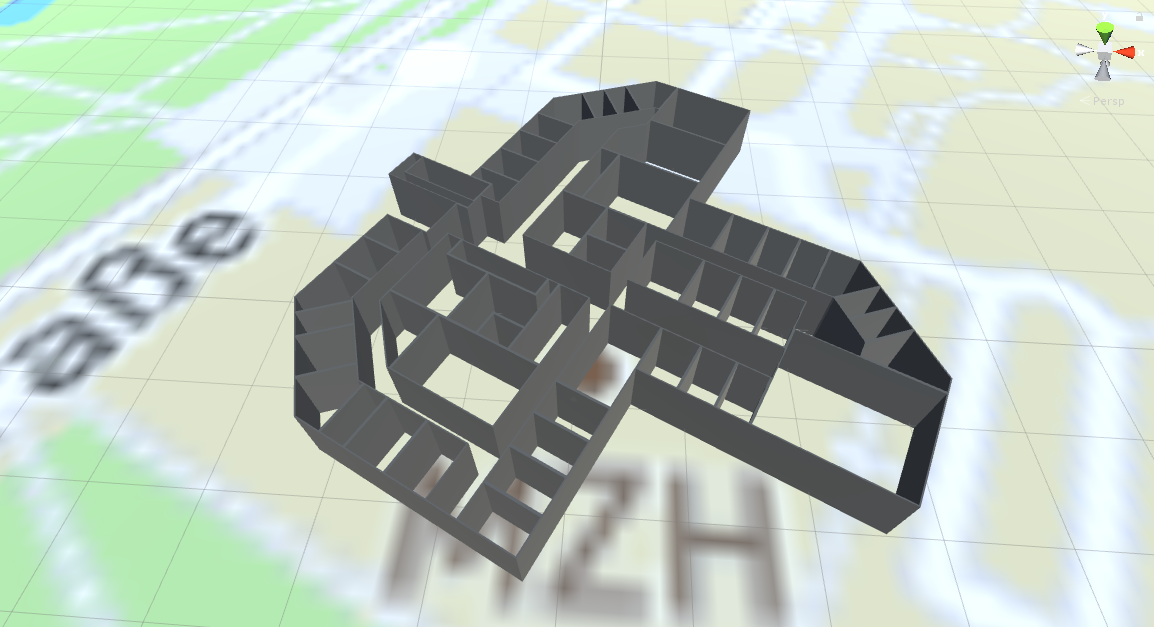
\includegraphics[width=\textwidth]{figures/mapbox_unity_mzh_e5_z15_working}
    \caption{3D-Darstellung des Lageplans der Ebene 5 im MZH.\@ %
    Nur die Wände werden hier angezeigt.}
    \label{fig:mapbox_unity_mzh_e5_z15}
\end{figure}

Im Verlauf einer ersten Implementierung einer Megamap basierend auf Mapbox ergaben sich Probleme, die auf die im Folgenden näher eingegangen wird.

\subsubsection*{Detailverlust und visuelle Artefakte bei unterschiedlichen Zoom-Ebenen}
Ein Nachteil beim zuvor genannten Ansatz ist, dass die erstellten Indoor-Polygone im Vergleich zu Gebäuden oder sogar ganzen Ländern sehr klein sind.
Die Breiten-/Längengrade der Vertices unterscheiden sich daher erst nach einigen Nachkommastellen.
Obwohl Mapbox intern die Koordinaten als 64-Bit-Werte repräsentiert \autocite{Kahyaoglu2017}, reicht bei einem niedrigen Zoom der Karte die Präzision zur Darstellung der Indoor-Objekte nicht aus.
\autoref{fig:mapbox_unity_mzh_e5_problems} zeigt das Problem auf mehreren Zoom-Stufen.
Bei einem niedrigen Zoom werden einige der Wände nicht gerendert, da vereinzelte Vertices nicht mehr unterschieden werden.
% TODO: Weiter ausführen... -> Github Issue

\begin{figure}
    \centering
    \begin{subfigure}{0.49\textwidth}
        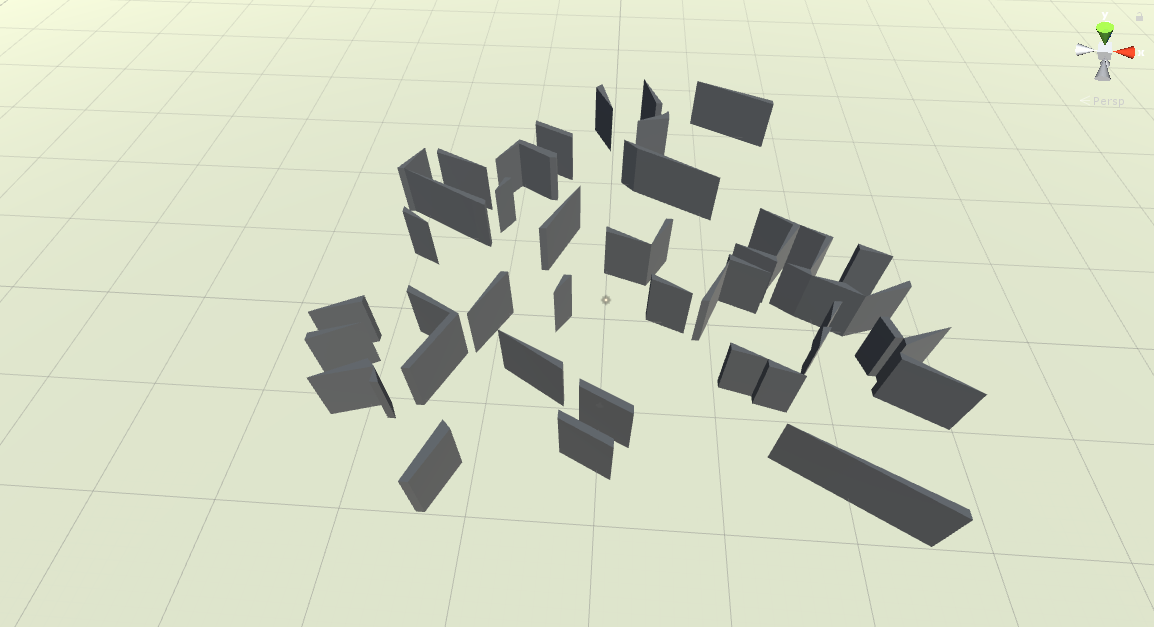
\includegraphics[width=\textwidth]{figures/mapbox_unity_mzh_e5_z9}
        \caption{\texttt{zoom = 9}}
        \label{sfig:mapbox_unity_mzh_e5_z9}
    \end{subfigure}
    \hfill
    \begin{subfigure}{0.49\textwidth}
        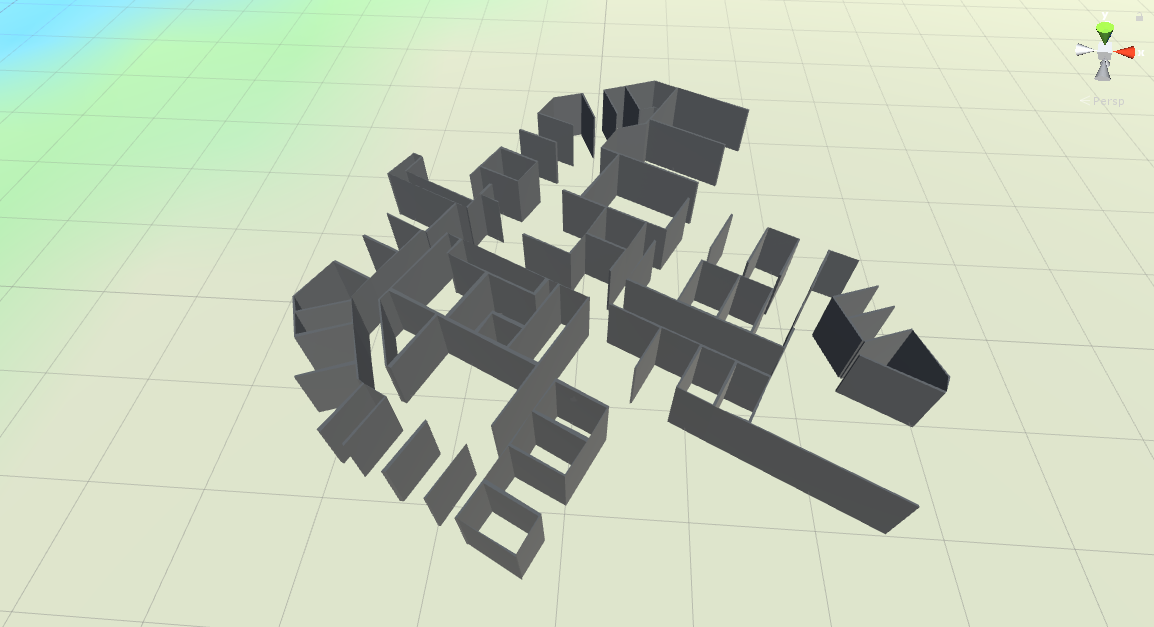
\includegraphics[width=\textwidth]{figures/mapbox_unity_mzh_e5_z11}
        \caption{\texttt{zoom = 11}}
        \label{sfig:mapbox_unity_mzh_e5_z11}
    \end{subfigure}
    \newline
    \begin{subfigure}{0.49\textwidth}
        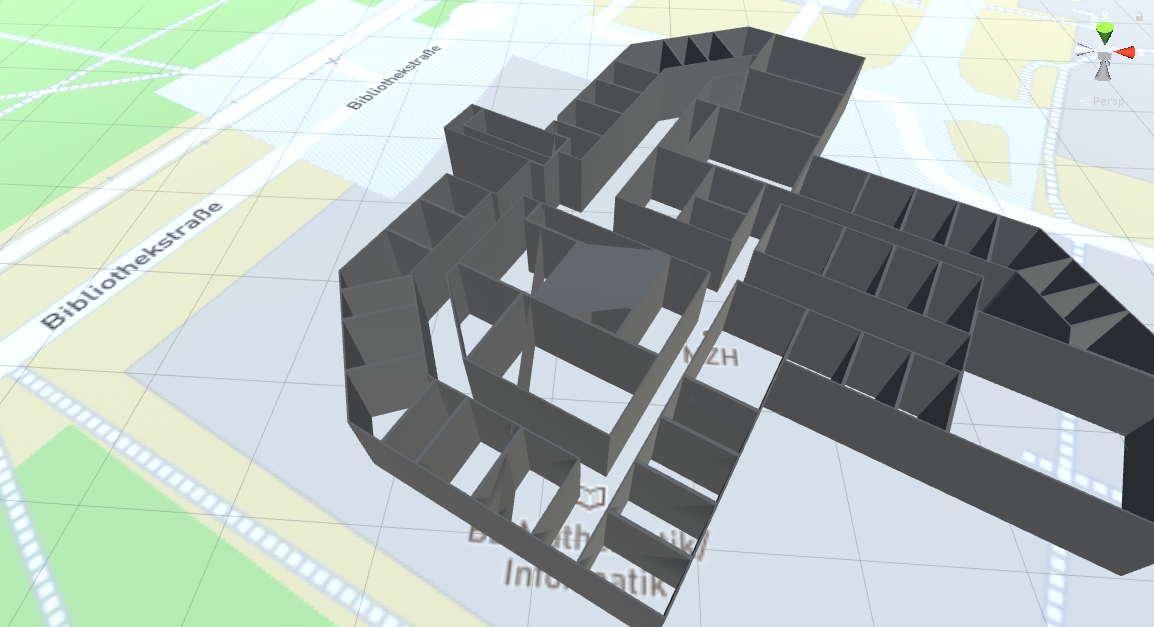
\includegraphics[width=\textwidth]{figures/mapbox_unity_mzh_e5_z18}
        \caption{\texttt{zoom = 18}}
        \label{sfig:mapbox_unity_mzh_e5_z18}
    \end{subfigure}
    \caption{Fehlende Wände und visuelle Artefakte bei unterschiedlichen Zoom-Ebenen.}
    \label{fig:mapbox_unity_mzh_e5_problems}
\end{figure}

Ein weiteres Problem ist, dass bei einem hohen Zoom visuelle Artefakte entstehen (siehe \autoref{sfig:mapbox_unity_mzh_e5_z18}).
Hier werden sowohl eine \enquote{Decke} als auch eine diagonale Wand eingezeichnet, die im originalen Datensatz nicht vorhanden sind.
Die Indoor-Karte befinden sich in diesem Fall auf der Schnittgrenze zweier Tiles.
Da Mapbox ein bekanntes Problem mit Gebäuden hat, die sich auf der Grenze mehrerer Tiles befinden, ist naheliegend, dass das Problem daher resultiert \autocite{Mapbox2018c}.

\subsubsection*{Ersetzung von OpenStreetMap-Gebäuden nicht möglich}
Wie bereits erwähnt ist in \autoref{fig:mapbox_unity_uni_bremen} der zentrale Gebäudekomplex der Universität Bremen abgebildet.
Die farblichen Markierungen zeigen jedoch, dass Teile mancher Gebäude (in diesem Fall das MZH und das GW2) fehlen.
Ein Gebäude kann in OSM durch die Zusammensetzung mehrerer Polygone definiert werden, um komplexere Strukturen wie z.B. unterschiedlich hohe Dachebenen darstellen zu können.
Die Technik wird auch für das MZH und das GW2 angewendet.
Es ist unklar, warum Teile des OSM-Datensatzes in Mapbox nicht angezeigt werden.
Zum Vergleich zeigt \autoref{fig:uni-bremen_osm2world}, wie die Gebäude eigentlich in der 3D-Darstellung aussehen sollten.
Für das Bild wurde direkt von OSM der entsprechende Ausschnitt der Uni exportiert und mit dem Programm \emph{OSM2World} gerendert.
Es wird deutlich, dass die Gebäudedaten in der Tat in der OSM-Datenbank vorhanden sind, weshalb das Fehlen dieser bei der Darstellung in Unity auf Mapbox zurückzuführen ist.

\begin{figure}
    \centering
    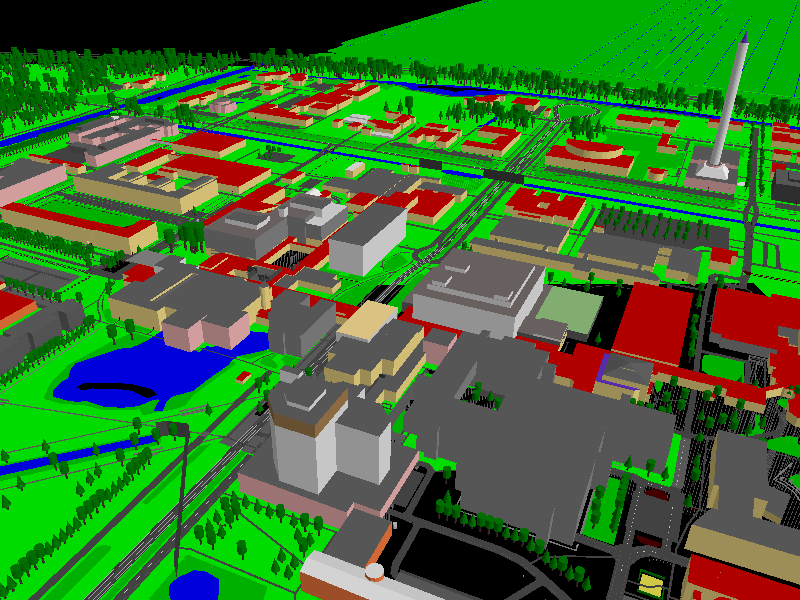
\includegraphics[width=\textwidth]{figures/uni-bremen_osm2world}
    \caption{Von OSM2World gerendertes Bild der Universität Bremen, basierend auf Daten aus OSM.\@ %
    Insbesondere das MZH und das GW2 werden korrekt dargestellt.%
    }
    \label{fig:uni-bremen_osm2world}
\end{figure}

Theoretisch wäre es möglich, das fehlerhafte Gebäudemodell durch ein korrigiertes zu ersetzen.
Mapbox bietet hierfür einen \texttt{ReplaceFeatureModifier} an.
Diesem kann ein Breiten- und Längengrad sowie ein Unity-Prefab übergeben werden.
Falls sich an den angegebenen Koordinaten ein Feature befindet (z.B. ein Gebäude), wird dieses gelöscht und stattdessen wird das Prefab auf der Karte platziert \autocite{Mapbox2018d}.

Allerdings funktioniert dieser \emph{Modifier} nur, wenn die \unity{AbstractMap} so eingestellt ist, dass nur Gebäude mit einer eindeutigen ID angezeigt werden.
Durch das Aktivieren dieser Einstellung werden jedoch in einigen Regionen, darunter auch Bremen, gar keine Gebäude angezeigt.
Werden wiederum die eindeutigen IDs für Gebäude nicht aktiviert, wirft Mapbox intern einen Fehler.
Dieser ist darauf zurückzuführen, dass nun für die betreffenden Gebäude sehr kurze IDs generiert werden (von 0 aufwärts gezählt) \autocite{Github2018}.

Folglich besteht keine Möglichkeit, die fehlerhaft generierten Gebäude zu entfernen und diese durch die korrigierten Varianten zu ersetzen.
Da außerdem die Darstellung der Indoor-Karte stark von den Einstellungen der \unity{AbstractMap} abhängt und wenig Kontrolle über die Visualisierung von Details wie Türen, Fenster oder Einrichtungsgegenstände bietet, wird das Mapbox SDK für die Implementierung einer Indoor-Megamap ausgeschlossen.

%
\cleardoublepage
